\documentclass{article}
\usepackage{longtable}
\usepackage{multirow}
\usepackage{array}
\usepackage{graphicx}  % For inserting images
\usepackage{caption}   % For better caption formatting
\usepackage{float}     % To control figure placement
\usepackage{booktabs}
\usepackage{array}
\usepackage{epsfig}
\usepackage{float}  % Allows better figure placement

\graphicspath{{fig/}} % Set the directory where graphics are located



\title{Artifact}
\author{Eduardo Oliveira}
\date{\today}

\begin{document}

\maketitle

\section{Open Science Platform}

\subsection{Overview}

Traditional centralized systems often exhibit data silos, limited verifiability, and susceptibility to manipulation, impeding the openness and reliability of scientific practices. The decentralized model introduced in this work is designed to mitigate these challenges by enabling efficient data sharing, fostering collaboration, and enhancing the validation of research outputs, thereby strengthening reproducibility and transparency.

This chapter details the design and implementation of the Open Science Platform, a decentralized system that integrates blockchain, IPFS, and smart contracts to improve research reproducibility. By leveraging immutable records and decentralized storage, the platform ensures transparent and verifiable research artifact management. Additionally, extended services are incorporated to facilitate file indexing, metadata extraction, and search functionality. The proposed platform aligns with Open Science principles by providing verifiable and persistently traceable access to research artifacts.


\begin{figure}[htbp]
      \centering
      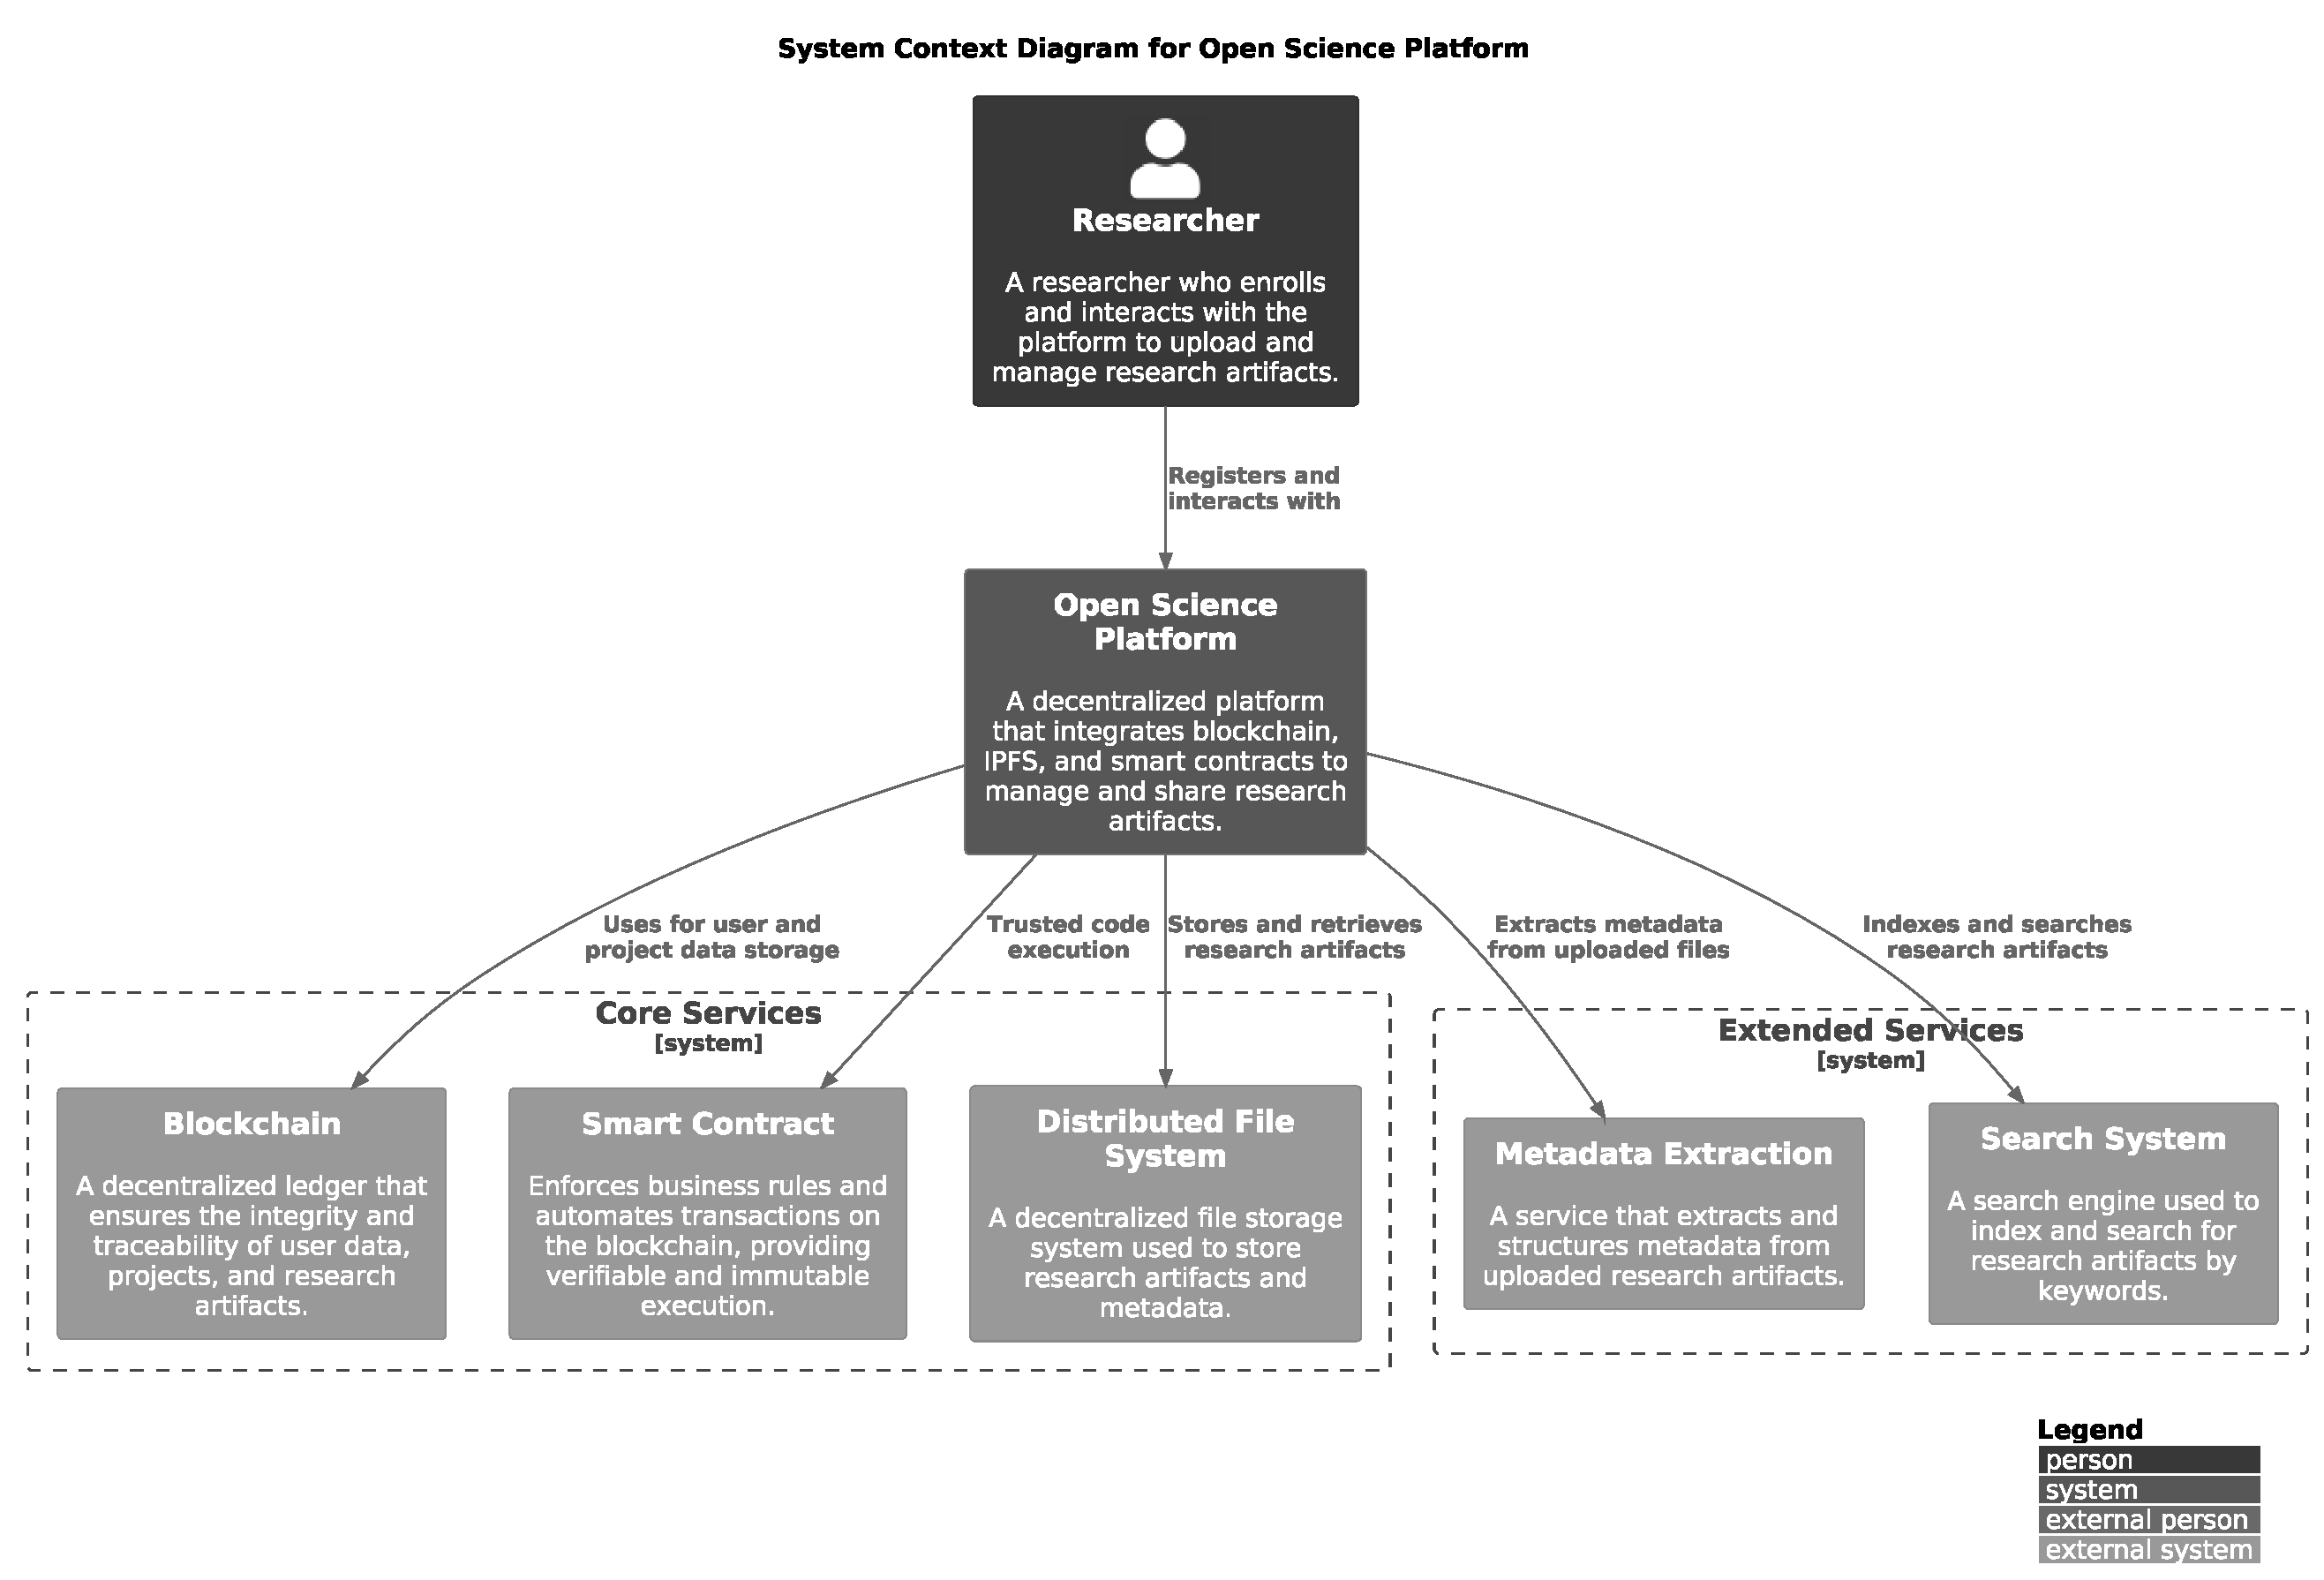
\includegraphics[width=0.98\textwidth, keepaspectratio]{c4_context_diagram}
      \caption{System context diagram for the Open Science Platform}
      \label{fig:c4_context_diagram}
\end{figure}



\subsection{Technology Stack}
The Open Science Platform is developed using a hybrid architecture that combines decentralized and off-chain technologies to ensure secure, traceable, and efficient data management.

\subsection{Core Services}

The core services of the Open Science Platform provide the fundamental infrastructure for secure and verifiable research artifact management.

\begin{itemize}
      \item \textbf{Hyperledger Iroha v1 Blockchain:} Acts as the core infrastructure for managing user and project accounts, recording transactions, and enforcing business rules via smart contracts to ensure secure and transparent data exchange.
      \item \textbf{InterPlanetary File System (IPFS):} Provides decentralized, tamper-proof storage for research artifacts and metadata, ensuring persistent and verifiable access to shared data.
\end{itemize}

\subsection{Extended Services}

The extended services enhance the platform's features by improving file and metadata processing.

\begin{itemize}
      \item \textbf{Apache Tika:} Extracts metadata from uploaded files, enhancing artifact organization and searchability.
      \item \textbf{Whoosh:} Facilitates efficient indexing and keyword-based search for stored artifacts.
\end{itemize}


\subsection{User Interface, integration and execution}

\begin{itemize}
      \item \textbf{Jupyter Notebooks (Python):} Powers the front-end interface, facilitating the automation and display of the execution steps. Blockchain interactions are managed via the Iroha v1 Python library, while communication with the IPFS network is handled through the HTTPS client library.
\end{itemize}

\begin{figure}[htbp]
      \centering
      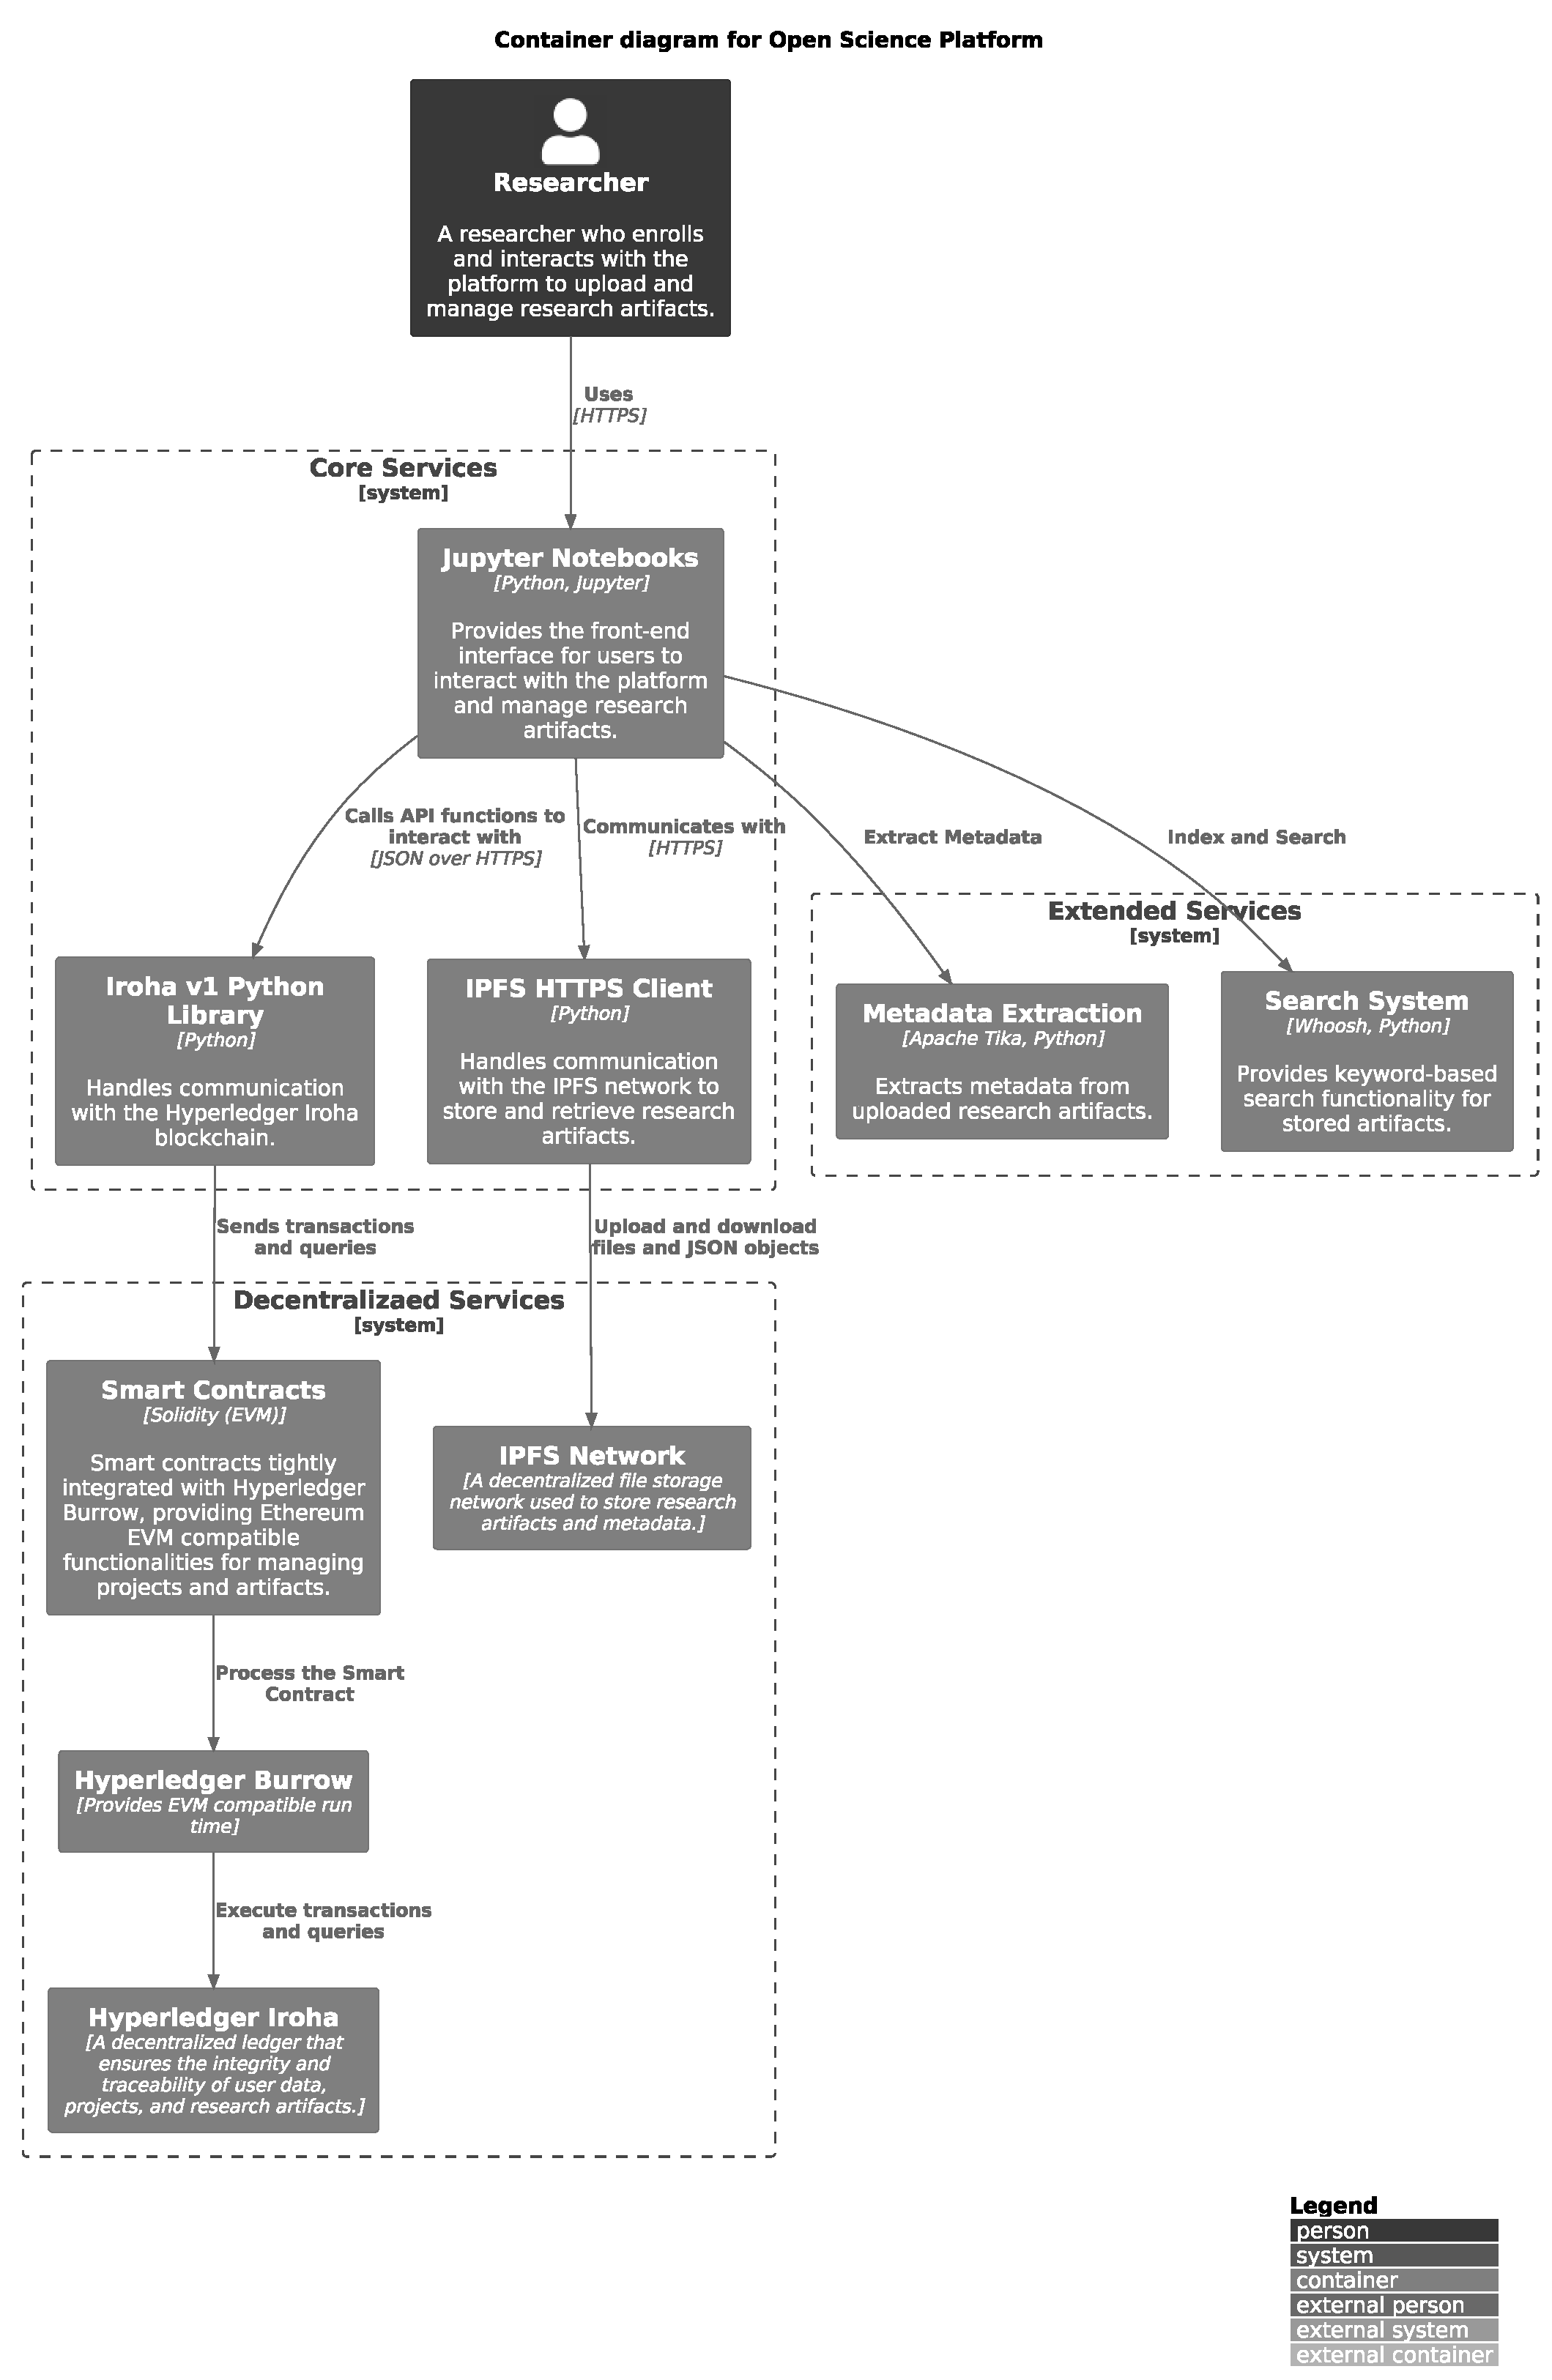
\includegraphics[width=0.98\textwidth, keepaspectratio]{c4_container_diagram}
      \caption{Container diagram for the Open Science Platform}
      \label{fig:c4_container_diagram}
\end{figure}



\subsection{Platform Operations}
The platform supports a set of core operations that regulate user interactions with projects and data management.

\begin{itemize}
      \item \textbf{User Self-Enrollment} – A user self-enrolls on the platform by providing a private key that complies with the ED25519 or SHA-3 standards and identity information, including full name, institution, email, ORCID, and role. An account is created for the user in the blockchain. All data provided in the enrollment is structured in key/value pairs into a JSON object and uploaded to IPFS, with the corresponding Content Identifier (CID) recorded on the blockchain attributes of the user account.

      \item \textbf{Project Registration} – Users can register a project by specifying a descriptive name, an abstract, relevant keywords, start and end dates, funding agency, and location. Upon registration, a blockchain account is created. This data is structured in key/value pairs into a JSON object and uploaded to IPFS, with the corresponding Content Identifier (CID) recorded on the blockchain attributes of the project account.


      \item \textbf{User and Project Accounts Linkage} – Once both user and project accounts are created, the system updates their attributes to establish a bidirectional association. This ensures that querying a user account reveals linked project accounts, and vice versa, facilitating traceability and efficient project management.
\end{itemize}


\begin{figure}[htbp]
      \centering
      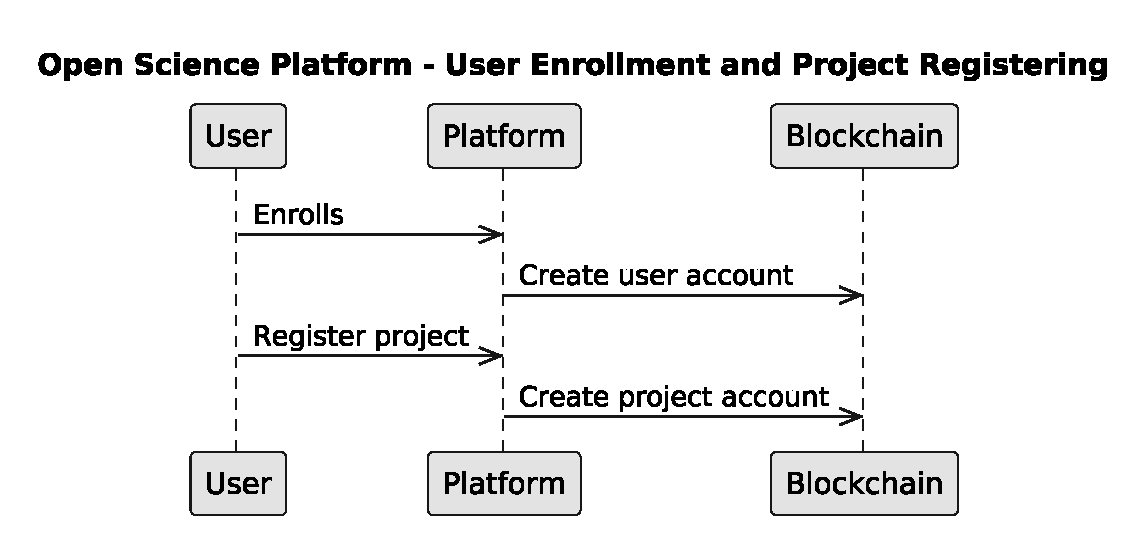
\includegraphics[width=0.98\textwidth, keepaspectratio]{c4_platform_operations_1}
      \caption{User enrollment and project registering for the Open Science Platform}
      \label{fig:c4_operations_diagram}
\end{figure}


\subsection{Artifact Management}

\begin{itemize}
      \item \textbf{File Upload} – A user may upload research artifacts, including papers, datasets, and images. Each file is stored on IPFS, generating a unique Content Identifier (CID) that ensures traceability and integrity. The CID is then recorded on the blockchain attributes of the project, establishing a verifiable reference to the artifact.

      \item \textbf{Metadata Extraction and Storage} – After the upload,the file available metadata is extracted. The extracted metadata is structured in key/value pairs into a JSON object and uploaded to IPFS, with the corresponding Content Identifier (CID) recorded on the attributes of the project account in the blockchain, ensuring metadata provenance and verification.

      \item \textbf{Indexing} – To facilitate efficient retrieval, the system indexes the metadata of every uploaded file, including full text indexing for text based files.

      \item \textbf{Searching} – Users can perform keyword-based searches to locate relevant research artifacts, with search results displaying metadata details, including descriptions, subject and authorship.
\end{itemize}


\begin{figure}[htbp]
      \centering
      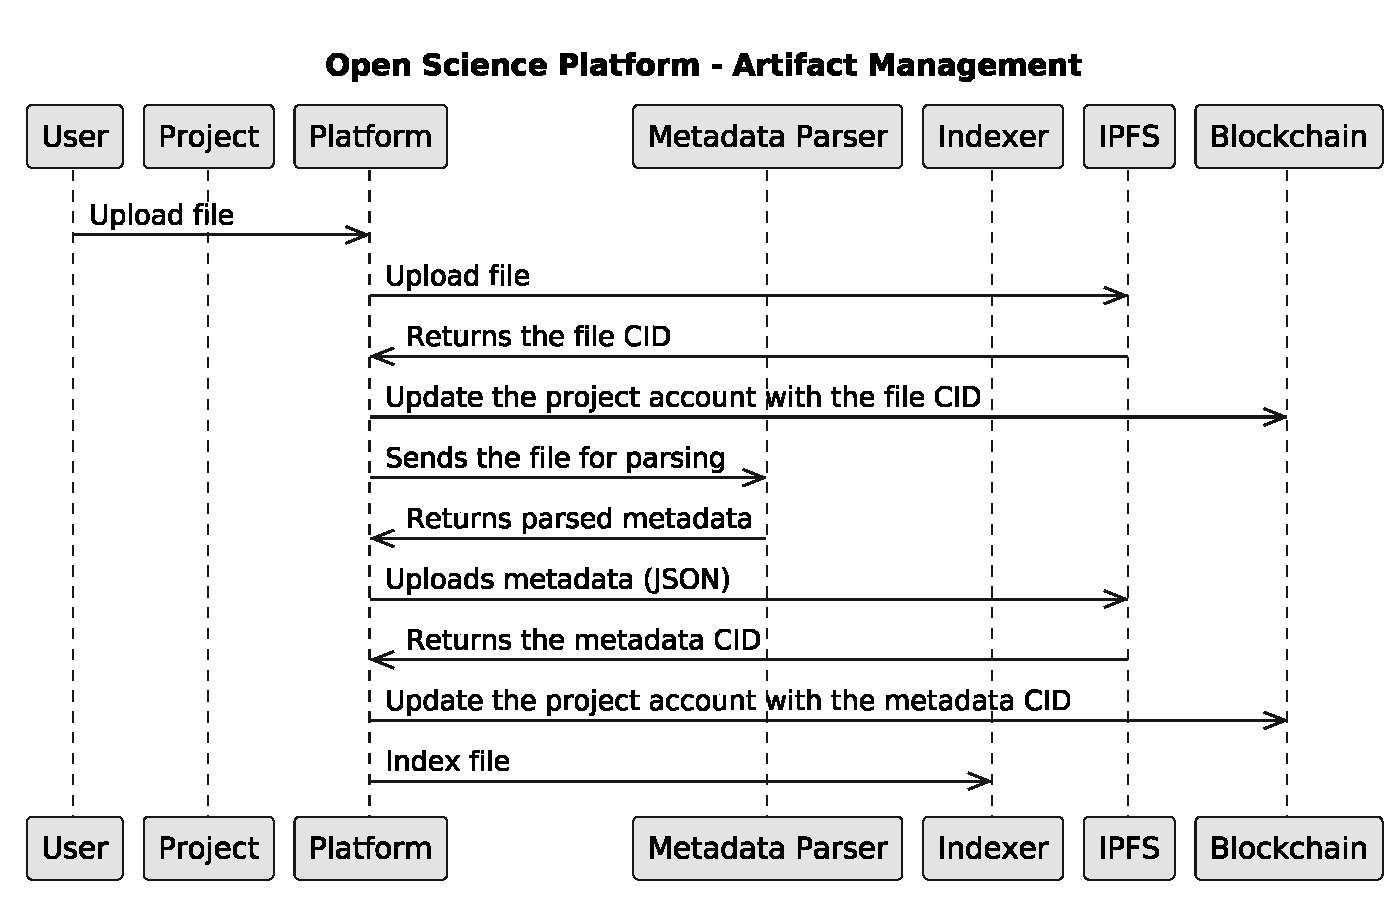
\includegraphics[width=0.98\textwidth, keepaspectratio]{c4_platform_operations_2}
      \caption{File operations diagram for the Open Science Platform}
      \label{fig:c4_file_operations_diagram}
\end{figure}



\subsection{Verification and Access}

\begin{itemize}
      \item \textbf{File Validation} – To ensure data integrity and authenticity, the platform verifies whether the CID of a file stored on IPFS matches the CID recorded on the blockchain. A discrepancy between these identifiers signals potential tampering or corruption.

      \item \textbf{File Download} – The system retrieves and downloads validated files from IPFS to the user local file system for later usage.
\end{itemize}


\subsection{Data Model}

The data model that supports the platform is comprised of two main classes User and Project. The User class contains attributes for user identity information, while the Project class contains attributes for project metadata. A many-to-many relationship exists between Users and Projects where, a single user can be associated with multiple projects.

To describe the attributes of each entity in the data model, three main ontologies were considered: FOAF (Friend of a Friend), Dublin Core and Schema.org. These standard vocabularies provide a common language for describing metadata information and can potentially easy the integration with other systems adopting W3C standards for semantic Web, like knowledge graphs, for instance.

\subsection{Entity-relationship model}


blokchains, smart contracts are verifiable piece of code

\subsection{Ontologies}

To describe the attributes of each entity in the data model, three main ontologies were considered: FOAF (Friend of a Friend), Dublin Core and Schema.org. These standard vocabularies provide a common language for describing metadata information and can potentially easy the integration with other systems adopting W3C standards for semantic Web, like knowledge graphs, for instance.

\subsection{Entity-relationship model}


blokchains, smart contracts are verifiable piece of code


\subsection{Metadata}

Metadata in the context of the platform has a two fold approach. The first is related to the identity of an user account, holding key value pairs of attributes related to the user such as full name, email, institution, ORCID.


\begin{verbatim}
      {
          "@context": {
              "schema": "http://schema.org/",
              "foaf": "http://xmlns.com/foaf/0.1/"
          },
          "@graph": [
              {
                  "@type": "foaf:Person",
                  "foaf:name": "Jolly Noether",
                  "foaf:mbox": "jolly_noether@email.com",
                  "foaf:organization": {
                      "@type": "foaf:Organization",
                      "foaf:name": "Morris College"
                  },
                  "schema:identifier": {
                      "@type": "PropertyValue",
                      "propertyID": "ORCID",
                      "value": "9833-6461-2701-X"
                  },
                  "foaf:holdsAccount": {
                      "schema:identifier": "jolly_noether@test",
                      "schema:roleName": "author",
                      "schema:publicKey": <publick ey value>},
                  "schema:linked_project": "10278@test"
              }
          ]
      }
      \end{verbatim}




\subsection{Smart Contract}

The platform deploys standard Ethereum EVM contracts in Solidity for account creation and detail setting. These contracts are deployed through the Iroha v1 Python Library.

\subsection{Benefits}

The Open Science platform offers numerous benefits for researchers and members of the scientific community, including:

\begin{itemize}
      \item Secure data sharing: By utilizing blockchain technology and IPFS, the platform ensures tamper-proof data exchange.
      \item Transparent data management: The use of smart contracts and decentralized storage guarantees transparency in data access and modification history.
      \item Collaborative research environment: The platform enables researchers to collaborate on projects, share artifacts and results, and track progress.
\end{itemize}

\subsection{Challenges}

The Open Science platform faces several challenges, including:

\begin{itemize}
      \item Scalability: As the number of users increases, the platform needs to be able to handle a growing amount of data and transactions efficiently.
      \item Interoperability: Ensuring seamless integration with existing research platforms and tools is crucial for widespread adoption.
      \item User Adoption: Educating researchers about the benefits of decentralized technologies and the Open Science platform can be an uphill battle.
\end{itemize}

\subsection{Future Work}

The Open Science platform has several areas for future development, including:

\begin{itemize}
      \item Integration with existing research platforms: Collaborations with established research platforms to expand the platform's reach and user base.
      \item Enhanced security measures: Implementing additional security protocols to protect against potential threats and maintain the integrity of shared information.
      \item User interface improvements: Enhancing the web interface to make it more user-friendly and accessible for researchers from diverse backgrounds.
\end{itemize}

\section{Conclusion}
The Open Science platform is a comprehensive solution for secure, transparent, traceable, and tamper-proof data sharing and collaboration. By leveraging decentralized technologies, the platform empowers researchers to share project artifacts and data in a reliable and trustworthy manner.

\end{document}



